% Fractal: un atlas interactivo de movilidad del metro de Nueva York
% Paper final del curso DS5343 Visualización de Datos (UTEC, 2026-2).
% Compilar:  pdflatex FinalPaper.tex  (dos veces). Las figuras están en figuras/ y sus fuentes en figuras/src/.
\documentclass[conference,a4paper]{IEEEtran}
\usepackage[utf8]{inputenc}
\usepackage[T1]{fontenc}
\usepackage[spanish,es-tabla,es-nodecimaldot,es-noquoting,es-noshorthands]{babel}
\usepackage{graphicx}
\usepackage{amsmath}
\usepackage{booktabs}
\usepackage{capt-of}
\usepackage{microtype}
\usepackage[hidelinks]{hyperref}
\graphicspath{{figuras/}}
\hypersetup{pdftitle={Fractal: un atlas interactivo de movilidad del metro de Nueva York},pdfauthor={Renzo Acervo Correa, Stewart Maquera Bobadilla}}
\renewcommand{\IEEEkeywordsname}{Palabras clave}
\hyphenation{Man-hat-tan Brook-lyn com-ple-jos com-ple-jo We-b-G-P-U}

% El resumen gráfico va debajo del título, a todo el ancho de la página.
\makeatletter
\let\fractal@maketitle\@maketitle
\renewcommand{\@maketitle}{\fractal@maketitle
  \begin{center}
  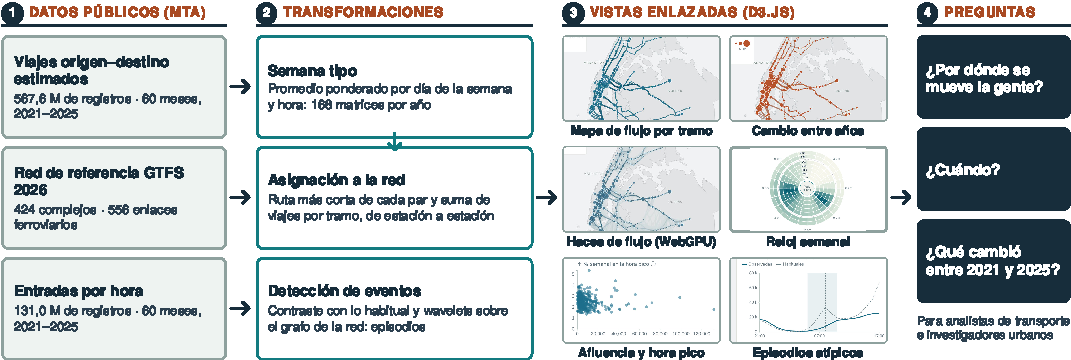
\includegraphics[width=\textwidth]{fig1_resumen_grafico.pdf}
  \captionsetup@fractal
  \end{center}\vspace{-0.9\baselineskip}}
\newcommand{\captionsetup@fractal}{\par\vspace{0.4\baselineskip}
  \parbox{\textwidth}{\footnotesize Figura~1.\ \textbf{Resumen gráfico.} De los datos a las preguntas: (1) partimos de tres fuentes públicas de la MTA;
  (2) las convertimos en una semana tipo por año, sumamos los viajes sobre los tramos de la red y detectamos episodios atípicos;
  (3) mostramos el resultado en vistas enlazadas hechas con D3.js; (4) las vistas responden tres preguntas de quien analiza la red.}}
\makeatother

\begin{document}

\title{Fractal: un atlas interactivo de movilidad\\ del metro de Nueva York}

\author{\IEEEauthorblockN{Renzo Acervo Correa \qquad Stewart Maquera Bobadilla}
\IEEEauthorblockA{DS5343 Visualización de Datos, Universidad de Ingeniería y Tecnología (UTEC), Lima, Perú\\
Aplicación: \url{https://stewartmb.github.io/data-visualization-2026-2/atlas/}}}

\maketitle
\setcounter{figure}{1}% la Figura 1 es el resumen gráfico, que va con el título

\begin{abstract}
El metro de Nueva York mueve unos 3,5 millones de viajes estimados por día, pero las entradas por estación no dicen por dónde pasan esos viajes ni cómo se reparten en la semana. Presentamos Fractal, una aplicación web hecha con D3.js que toma las estimaciones origen--destino que publica la MTA para 2021--2025 (567,6 millones de registros), las suma sobre los tramos de la red y las muestra en vistas enlazadas: un mapa de flujo por tramo, mapas pequeños por año, un reloj semanal de $7\times24$ celdas, un diagrama de dispersión de complejos y una vista de episodios atípicos. Con ella vemos que los viajes crecieron 69\,\% entre 2021 y 2025, que el crecimiento fue desigual entre boroughs (+89\,\% en Manhattan frente a +23\,\% en el Bronx) y que desde los otros boroughs subió la proporción de viajes con destino en Manhattan.
\end{abstract}

\begin{IEEEkeywords}
movilidad urbana, datos origen--destino, vistas enlazadas, agrupamiento de aristas, D3.js
\end{IEEEkeywords}

\section{Introducción}
La MTA publica cuántas personas entran a cada estación del metro por hora. Ese dato dice cuánta gente entra, pero no a dónde va. Desde hace poco publica también una estimación origen--destino (OD): para cada mes, día de la semana y hora, el promedio de viajes entre cada par de complejos de estaciones. Es difícil de usar tal como viene: son 567,6 millones de filas para 2021--2025 y, con 424 complejos, hay hasta 179\,352 pares posibles en cada hora. Una línea por par tapa el mapa, y una tabla de ese tamaño no se puede explorar.

Fractal está pensado para analistas de transporte e investigadores urbanos que necesitan saber \emph{por dónde} se mueve la gente, \emph{cuándo} lo hace y \emph{qué cambió} entre 2021 y 2025. Corre en el navegador, sin instalar nada.

Nuestras contribuciones son tres: (1) un proceso reproducible que va de los datos de la MTA a 840 matrices OD (5 años $\times$ 168 horas de la semana) y a la carga de cada tramo; (2) una aplicación en D3.js con vistas enlazadas que responde las tres preguntas, con haces de flujo opcionales calculados en la GPU; y (3) una adaptación de la detección de eventos con wavelets sobre grafos a las entradas por hora.

\section{Trabajo relacionado}
\textbf{Flujos origen--destino.} Los mapas de flujo con una línea por par se saturan rápido. Los OD maps~\cite{odmaps} evitan las líneas anidando mapas pequeños, pero pierden la red. El agrupamiento de aristas junta líneas parecidas~\cite{fdeb,kdeeb}, aunque los haces pueden pasar por donde no existe ninguna ruta. RAEB~\cite{raeb} corrige eso guiando los haces con una jerarquía de la red vial. Adaptamos RAEB al metro, pero no como vista principal: ahí los viajes solo van por las vías, y sumar por tramo ya responde por dónde pasan. Para el tiempo, Dhont et al.~\cite{clock} ordenan días y horas en anillos y sectores; de ahí sale nuestro reloj semanal.

\textbf{Eventos en datos espaciotemporales.} ManyWaves~\cite{manywaves} usa la transformada wavelet sobre grafos~\cite{hammond} para resaltar cambios bruscos en datos multivariados. La aplicamos a una sola señal: la diferencia entre las entradas observadas y las habituales.

\textbf{Comparación y vistas coordinadas.} Gleicher et al.~\cite{comparison} distinguen entre yuxtaponer, superponer y codificar la diferencia; usamos lo primero en los mapas por año y lo último al comparar dos años.

\section{Tareas de análisis}
Definimos siete tareas que guiaron el diseño. Siguen la tipología de Brehmer y Munzner~\cite{tasks}. T1--T2 responden \emph{por dónde}, T3--T4 \emph{cuándo} y T5--T7 \emph{qué cambió}.

\noindent\textbf{T1 Actividad y tránsito.} Localizar los complejos con más actividad y los tramos con más carga.\\
\textbf{T2 Destinos y conexiones.} Identificar a dónde van las salidas de un complejo o de una zona.\\
\textbf{T3 Franja y destinos.} Comparar las salidas de un complejo entre franjas de la semana.\\
\textbf{T4 Concentración semanal.} Comparar cuánto concentra cada complejo en su hora pico.\\
\textbf{T5 Volumen y ritmo.} Comparar el volumen y el perfil semanal de un complejo entre dos años.\\
\textbf{T6 Cambio de destinos.} Identificar qué destinos ganaron o perdieron viajes entre dos años.\\
\textbf{T7 Desviaciones.} Localizar horas fuera de lo habitual, su duración y los complejos que más aportan.

\section{Datos y métodos}
\subsection{Datos}
La Tabla~\ref{tab:datos} resume las fuentes, todas públicas. La matriz OD es una \emph{estimación} de la MTA, no un registro de viajes: en el metro se valida al entrar, no al salir, y la MTA infiere el destino. Las entradas por hora también son estimaciones que publica la MTA, pero con fecha y hora concretas; las llamamos \emph{observadas} para distinguirlas de las habituales. Sus 131 millones de filas son los archivos originales, con todos los modos de transporte: el detector usa solo las del metro.

\begin{table}[t]
\caption{Fuentes de datos (MTA, portal Open NY)}
\label{tab:datos}
\centering\footnotesize
\begin{tabular}{@{}p{0.33\columnwidth}p{0.33\columnwidth}p{0.24\columnwidth}@{}}
\toprule
Fuente & Contenido & Tamaño\\
\midrule
Estimación OD del metro, 2021--2025~\cite{data} & Viajes promedio por par, mes, día de la semana y hora & 567\,608\,985 filas (60 meses)\\
Entradas por hora, 2021--2025~\cite{data} & Entradas por complejo y hora & 130\,987\,497 filas\\
GTFS de referencia, 2026 & Paradas, vías y transbordos & 475 paradas, 556 enlaces, 75 transbordos\\
\bottomrule
\end{tabular}
\end{table}

\begin{figure*}[t]
\centering
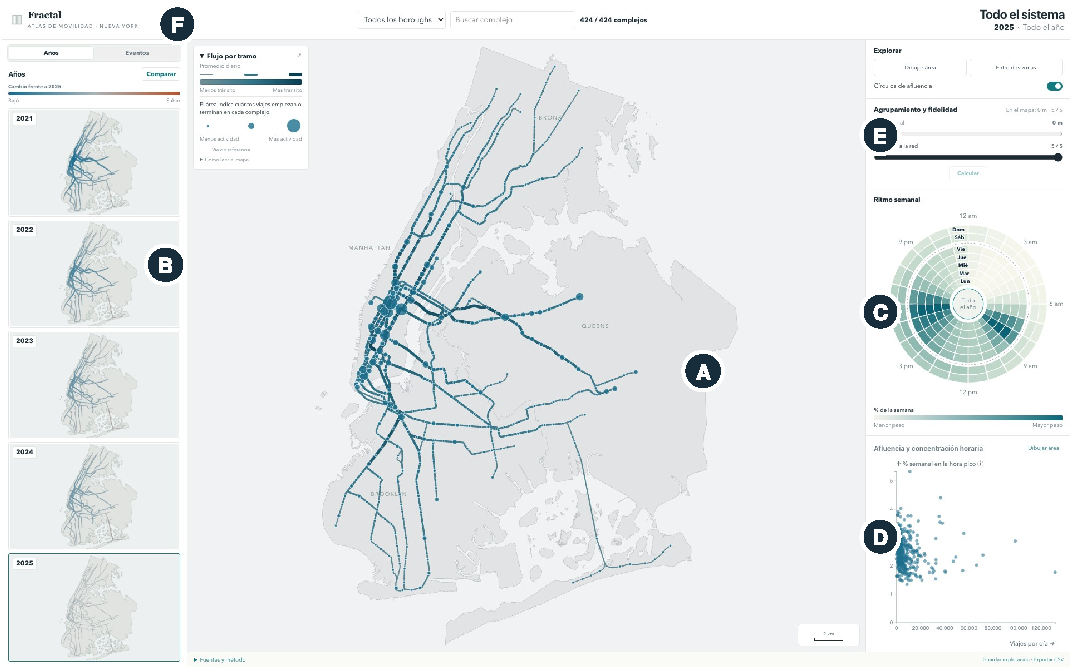
\includegraphics[width=0.58\textwidth]{fig2_app.pdf}
\caption{Vista principal de Fractal. (A) Mapa de flujo por tramo; (B) mapas pequeños por año; (C) reloj semanal; (D) dispersión de complejos; (E) exploración y control de los haces; (F) pestaña \emph{Eventos}, que reemplaza a (B) por el calendario de episodios.}
\label{fig:app}
\end{figure*}

\subsection{Semana tipo}
La MTA publica un promedio por mes. Para tener un año comparable calculamos una \emph{semana tipo}: para cada par $(i,j)$, día de la semana $d$ y hora $h$,
\begin{equation}
q_{ij}(d,h)=\frac{\sum_{m} n_m(d)\,a^{m}_{ij}(d,h)}{\sum_{m} n_m(d)},
\end{equation}
donde $a^{m}_{ij}$ es el promedio publicado para el mes $m$ y $n_m(d)$ es el número de veces que el día $d$ cae en ese mes. El resultado son 168 matrices de $424\times424$ por año, 840 en total, más un promedio diario anual.

\subsection{Métricas de comparación}
Para un complejo, $p_k$ es la parte de sus salidas de la semana tipo que cae en la franja $k$ (de 168). Su \emph{concentración máxima} es $100\max_k p_k$: el peso de su hora más cargada. Entre un año $A$ y un año $B$, el \emph{índice de volumen} es $100\,V_B/V_A$, con $V$ las salidas diarias, y el cambio de ritmo se mide con la variación total~\cite{tv}, en puntos porcentuales (pp):
\begin{equation}
\mathrm{TV}=50\sum_{k=1}^{168}\lvert p_{B,k}-p_{A,k}\rvert .
\end{equation}
El índice dice cuánto cambió la cantidad de viajes; la TV, cuánto cambió su reparto en la semana.

\subsection{Asignación a la red}
La demanda está por complejo (424), pero la red del GTFS está por parada: 475 paradas, 556 enlaces ferroviarios y 75 transbordos declarados. Un complejo agrupa una o más paradas, y un viaje puede salir o llegar por cualquiera de las suyas. A cada par le asignamos el camino de menor costo: cada enlace cuesta su longitud y cada transbordo, su tiempo mínimo declarado convertido a distancia a 8~m/s. Esa conversión es un supuesto nuestro. La carga de un tramo es la suma de los viajes cuyos caminos pasan por él. Los cinco años se asignan sobre la misma red de 2026 para que las diferencias entre años vengan de la demanda y no de cambios en el grafo. Son rutas modeladas, no observadas.

\subsection{Haces de flujo}
Para ver pares OD completos adaptamos RAEB~\cite{raeb}. Cada enlace recibe una importancia según su longitud, tipo y flujo, y el control de \emph{fidelidad} decide qué parte de la red guía los haces: 5, 10, 20, 40 o 100\,\% de los enlaces. Las curvas se juntan con iteraciones de KDEEB~\cite{kdeeb} hasta que dos imágenes seguidas se parecen lo suficiente (información mutua normalizada $\geq 0{,}8$) o se llega a 150 iteraciones. El cálculo corre en WebGPU, con respaldo en CPU y WebGL2.

\subsection{Transformada wavelet sobre el grafo}
Seguimos el fundamento de ManyWaves~\cite{manywaves}: wavelets sobre un grafo para resaltar cambios bruscos. La referencia semanal y las reglas para formar episodios son adaptaciones nuestras.

\emph{Señal.} Para cada complejo y hora, el valor habitual $u$ es la mediana de la misma hora y el mismo día de la semana en las cuatro semanas anteriores y posteriores. La diferencia con lo observado $o$ se mide como $c=2\,(\sqrt{o+3/8}-\sqrt{u+3/8})$, que atenúa el peso de las estaciones grandes.

\emph{Grafo y filtro.} Cada nodo es un complejo en una hora. El grafo une complejos vecinos (424 complejos y 549 conexiones, tras juntar las paradas de cada complejo) y horas consecutivas. Aplicamos wavelets de Hammond~\cite{hammond} (cuatro escalas, Chebyshev de orden 30) y nos quedamos con la banda de mayor frecuencia. La \emph{señal espectral} que muestra la aplicación es la magnitud de ese coeficiente dividida entre su rango intercuartílico, pasada por $\log(1+x)$ y dividida entre el máximo global: un valor entre 0 y 1, sin unidades.

\emph{Episodios.} El corte es el percentil 80 de los máximos de cada complejo en el periodo, el criterio de resaltado de ManyWaves. En cada hora agrupamos al menos tres complejos conectados que lo superan; los grupos de horas seguidas se unen si comparten al menos dos complejos. Un \emph{episodio} dura dos horas o más, y guardamos hasta seis por mes.



\section{Fractal: diseño de la visualización}
\subsection{Componentes visuales}
Fractal tiene seis componentes enlazados (Fig.~\ref{fig:app}) que comparten el mismo estado: año, hora de la semana y selección. Las vistas son SVG generado con D3~v7.9~\cite{d3} (los mapas pequeños usan canvas) y el sitio es estático: lee las matrices ya calculadas.

\textbf{(A) Mapa de flujo por tramo} (T1, T2). Cada tramo entre dos estaciones es una línea. El grosor y el color, en una escala secuencial de un solo tono, muestran los viajes por día que pasan por él. El área de cada círculo indica los viajes que empiezan o terminan en ese complejo. Al pasar el cursor aparece el valor exacto, y un clic en un complejo deja solo los viajes que salen de él.

\textbf{(B) Mapas pequeños por año} (T5, T6). Cinco mapas, de 2021 a 2025, muestran la diferencia de cada tramo frente al año abierto, con una escala divergente común (azul si bajó, terracota si subió). Con \emph{Comparar} se eligen dos años $A$ y $B$ y todas las vistas pasan a mostrar la diferencia (Fig.~\ref{fig:hallazgos}): en el mapa, el color de tramos y círculos indica si los viajes subieron o bajaron y el área del círculo, cuánto cambiaron hacia ese destino; el reloj muestra qué franjas ganaron o perdieron peso, en pp; y la dispersión pasa a índice de volumen frente a TV.

\begin{figure}[t]
\centering
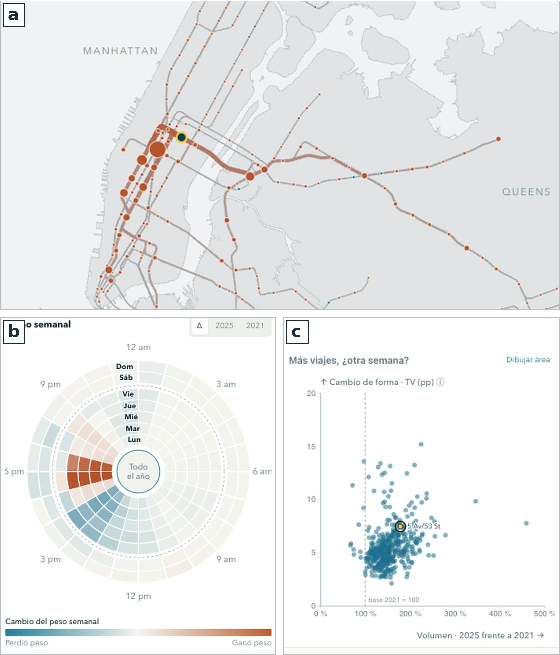
\includegraphics[width=0.52\columnwidth]{fig3_ritmo.pdf}
\caption{Comparación de 2021 ($A$) con 2025 ($B$) para 5~Av/53~St, promedio de todo el año. (a) Mapa: terracota si los viajes subieron y azul si bajaron; el área de cada círculo es el cambio de viajes hacia ese destino. (b) Reloj de diferencias: franjas que ganaron o perdieron peso en la semana. (c) Dispersión: índice de volumen frente a TV; el punto resaltado es 5~Av/53~St.}
\label{fig:hallazgos}
\end{figure}

\begin{figure*}[t]
\centering
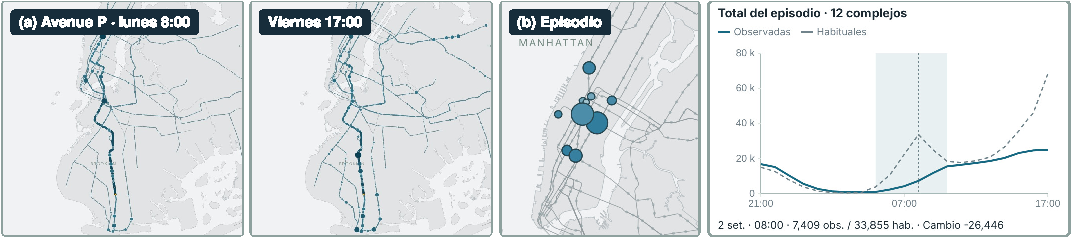
\includegraphics[width=0.86\textwidth]{fig4_casos.pdf}
\caption{Dos casos de uso. (a) Salidas de Avenue~P en 2025: el lunes a las 8:00 y el viernes a las 17:00; el mapa deja solo los tramos que usan esos viajes. (b) Episodio del 2 de septiembre de 2024 (Labor Day): complejos afectados a las 8:00 y entradas observadas frente a las habituales.}
\label{fig:casos}
\end{figure*}

\textbf{(C) Reloj semanal} (T3). Siete anillos, uno por día, y 24 sectores, uno por hora. El color indica qué porcentaje de los viajes de la semana cae en cada celda. Un clic en una celda lleva toda la aplicación a esa hora.

\textbf{(D) Dispersión} (T4, T5). Un punto por complejo: salidas por día en el eje horizontal y, en el vertical, su concentración máxima.

\textbf{(E) Exploración y haces} (T2). Se puede dibujar un área para quedarse con sus complejos, o dos para ver solo los viajes entre ellas. Incluye el radio y la fidelidad de los haces.

\textbf{(F) Eventos} (T7). Un calendario de años por meses resume la señal. Al elegir un episodio, el mapa marca los complejos afectados y una serie compara las entradas observadas con las habituales.

\subsection{Justificación del diseño}
\emph{Tramos en vez de líneas OD.} Muchos pares comparten las mismas vías, así que sumar por tramo reduce 179\,352 pares posibles a 556 marcas y responde directamente por dónde pasa la gente. Con líneas o haces como vista principal el mapa no se podía leer.

\emph{Haces opcionales.} Los tramos esconden qué pares hay detrás de un flujo, y los haces lo recuperan. Pero son una abstracción, no rutas: por eso se calculan solo al pulsar \emph{Calcular}.

\emph{Reloj circular.} La semana es cíclica y el reloj sirve de gráfico y de filtro; como las celdas de afuera son más grandes, el valor va en el color y no en el área.


\section{Resultados y casos de estudio}
\subsection{Crecimiento desigual y más destinos en Manhattan}
Los viajes estimados pasaron de 2,1 millones por día en 2021 a 3,5 millones en 2025 (+69\,\%). Por borough de origen, Manhattan creció 89\,\%, Brooklyn 57\,\%, Queens 54\,\% y el Bronx solo 23\,\%. En los tres boroughs que rodean Manhattan subió además la parte de los viajes que termina ahí: de 42,1 a 46,5\,\% en Brooklyn, de 47,1 a 50,1\,\% en Queens y de 53,5 a 56,3\,\% en el Bronx. Es un cambio en la proporción de destinos, no una medida de dependencia operativa.

\subsection{Volumen y ritmo no cambian igual (T5)}
En 5~Av/53~St las salidas diarias pasaron de 6357 a 11\,346 entre 2021 y 2025: un índice de volumen de 178,5 (Fig.~\ref{fig:hallazgos}c). Su semana también cambió, con una TV de 7,44~pp. El reloj de diferencias (Fig.~\ref{fig:hallazgos}b) muestra dónde: ganaron peso las horas cercanas a las 17:00 de los días laborales y lo perdieron las del inicio de la tarde. La hora más cargada sigue siendo el martes a las 17:00, pero pasó de 4,21 a 5,33\,\% de la semana. La dispersión separa así dos cosas que un solo número mezclaría: cuánto creció un complejo y cuánto cambió su horario.

\subsection{Dónde y cuándo se concentra (T1, T4)}
En 2025 el tramo más cargado es Bryant Pk $\leftrightarrow$ 34~St--Herald Sq, con 294\,385 viajes por día sumando ambos sentidos. El complejo con más actividad es Times Sq--42~St: 260\,005 viajes empiezan o terminan ahí. En la dispersión, 5~Av/53~St concentra el 5,33\,\% de su semana en una sola hora (martes a las 17:00); Christopher~St, con un volumen parecido, solo el 1,34\,\%.

\subsection{Caso 1: los destinos de una estación (T2, T3)}
Elegimos Avenue~P, una estación del sur de Brooklyn, y en el reloj el lunes a las 8:00 (Fig.~\ref{fig:casos}a). El mapa deja solo sus salidas: 296 viajes en esa hora, de los que el 53,9\,\% termina en Manhattan. Al pasar al viernes, la misma estación tiene 258 salidas a las 8:00 y solo 92 a las 17:00, y Manhattan baja de 48,1 a 25,7\,\% de los destinos: por la tarde el primer destino es Church~Av, dentro de Brooklyn. Son promedios del año, no días concretos.

\subsection{Caso 2: el Labor Day de 2024 (T7)}
El detector encontró 147 episodios en 49 de los 60 meses. Uno de los más claros es el del lunes 2 de septiembre de 2024 (Fig.~\ref{fig:casos}b): entre las 5:00 y las 10:00, doce complejos de Manhattan tuvieron muchas menos entradas que un lunes normal. A las 8:00 entraron 7409 personas donde suelen entrar 33\,855 ($-$78\,\%). Era feriado: el detector no sabe de feriados y aun así marcó los cinco Labor Day del periodo.

\section{Discusión}
\textbf{Qué aprendimos.} Que la unidad de agregación importa más que el tipo de gráfico: el proyecto mejoró cuando dejamos de dibujar pares y empezamos a sumar por tramo.

\textbf{Fortalezas.} Todo sale de datos públicos, se reproduce con los scripts del repositorio y corre en el navegador, sin servidor.

\textbf{Limitaciones.} La matriz OD es una estimación de la MTA y heredamos sus errores. Las rutas son el camino de menor costo sobre la red de 2026: no consideran la congestión ni los cambios de servicio de cada año. La carga de un tramo no indica saturación: faltan capacidad y frecuencia. Un episodio es una desviación por revisar, no su causa; el percentil 80 y las reglas de agrupación son decisiones nuestras, sin validar contra un registro de incidentes. Sin WebGPU los haces son bastante más lentos; no medimos los tiempos de forma sistemática.

\textbf{Evaluación informal.} No hicimos un estudio formal con usuarios. En la revisión del 14 de octubre el profesor pidió más protagonismo para los gráficos, menos texto y contexto geográfico: por eso el mapa ocupa el centro y el fondo muestra los boroughs. Al usarla vimos que costaba quitar una selección y que los haces en CPU eran lentos; de ahí salieron la tecla Escape y la versión en WebGPU.

\section{Trabajo futuro y conclusión}
Faltan una evaluación con analistas de transporte, asignar cada año sobre la red que estaba en servicio y cruzar los episodios con las alertas de la MTA.

Fractal muestra que una matriz origen--destino de cientos de millones de filas se puede explorar en el navegador si antes se la lleva al tramo de la red y a la hora de la semana.

\textbf{Agradecimientos.} Al profesor del curso por sus revisiones. Usamos asistentes de IA como apoyo en parte del código y del texto; revisamos y probamos todo.

\begin{thebibliography}{99}
\footnotesize
\bibitem{odmaps} J. Wood, J. Dykes y A. Slingsby, ``Visualisation of Origins, Destinations and Flows with OD Maps,'' \emph{The Cartographic Journal}, vol.~47, n.º~2, pp.~117--129, 2010.
\bibitem{fdeb} D. Holten y J. J. van Wijk, ``Force-Directed Edge Bundling for Graph Visualization,'' \emph{Computer Graphics Forum}, vol.~28, n.º~3, pp.~983--990, 2009.
\bibitem{kdeeb} C. Hurter, O. Ersoy y A. Telea, ``Graph Bundling by Kernel Density Estimation,'' \emph{Computer Graphics Forum}, vol.~31, n.º~3, pp.~865--874, 2012. doi:10.1111/j.1467-8659.2012.03079.x
\bibitem{raeb} W. Zeng, Q. Shen, Y. Jiang y A. Telea, ``Route-Aware Edge Bundling for Visualizing Origin-Destination Trails in Urban Traffic,'' \emph{Computer Graphics Forum}, vol.~38, n.º~3, pp.~581--593, 2019. doi:10.1111/cgf.13712
\bibitem{clock} M. Dhont, E. Tsiporkova, T. Tourwé y N. González-Deleito, ``Visual Analytics for Extracting Trends from Spatio-temporal Data,'' en \emph{Advanced Analytics and Learning on Temporal Data}, LNCS 12588, pp.~122--137, 2020. doi:10.1007/978-3-030-65742-0\_9
\bibitem{manywaves} G. Valdrighi, G. Garcia-Zanabria, M. Diaz, L. G. Nonato, N. Ferreira y J. Poco, ``ManyWaves: A Visual Analytics Approach for Exploring Multivariate Spatiotemporal Data Based on the Graph Wavelet Transform,'' \emph{Computer Graphics Forum}, 2026. doi:10.1111/cgf.70653
\bibitem{hammond} D. K. Hammond, P. Vandergheynst y R. Gribonval, ``Wavelets on Graphs via Spectral Graph Theory,'' \emph{Applied and Computational Harmonic Analysis}, vol.~30, n.º~2, pp.~129--150, 2011.
\bibitem{comparison} M. Gleicher, D. Albers, R. Walker, I. Jusufi, C. D. Hansen y J. C. Roberts, ``Visual Comparison for Information Visualization,'' \emph{Information Visualization}, vol.~10, n.º~4, pp.~289--309, 2011.
\bibitem{tasks} M. Brehmer y T. Munzner, ``A Multi-Level Typology of Abstract Visualization Tasks,'' \emph{IEEE Trans. Visualization and Computer Graphics}, vol.~19, n.º~12, pp.~2376--2385, 2013.
\bibitem{tv} J. Fredriksson y A. Karlström, ``A Fully Neural Network-Based Travel Demand and Scheduling Model, Covering Activities, Destinations, and Modes of Transportation,'' \emph{Data Science for Transportation}, vol.~7, art.~28, 2025. doi:10.1007/s42421-025-00141-5
\bibitem{d3} M. Bostock, V. Ogievetsky y J. Heer, ``D\textsuperscript{3}: Data-Driven Documents,'' \emph{IEEE Trans. Visualization and Computer Graphics}, vol.~17, n.º~12, pp.~2301--2309, 2011.
\bibitem{data} Metropolitan Transportation Authority, ``MTA Subway Origin-Destination Ridership Estimate'' (2021--2025) y ``MTA Subway Hourly Ridership'', Open NY, \url{https://data.ny.gov}. Conjuntos rapa-97zv, nqnz-e9z9, uhf3-t34z, jsu2-fbtj, y2qv-fytt, wujg-7c2s y 5wq4-mkjj. Consultado en 2026.
\end{thebibliography}

\end{document}
